\subsection*{Q3B}
Modelling a TBI as disturbing autoregulation to 50\% of its normal value, that is kGaut = 0.5; and an increase in CBF outflow (kRo) to 3.
\begin{figure}[h]
    \centering
    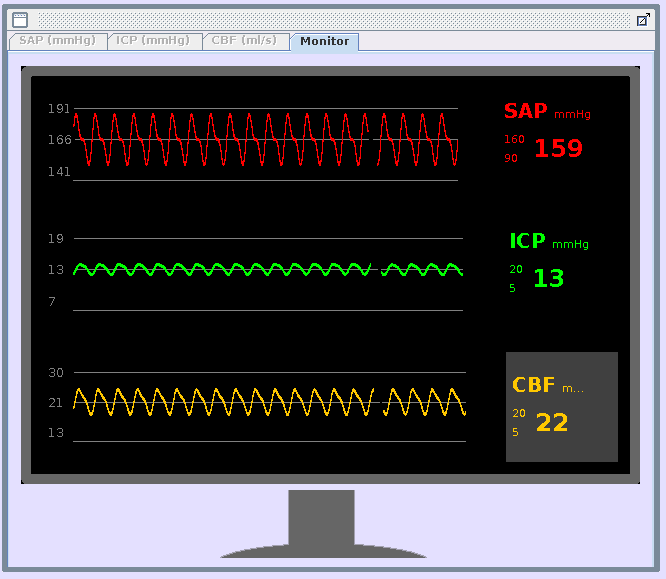
\includegraphics[width=0.7\textwidth]{images/Q3B-TBI.png}
    \caption{Brain injury -- kRo: 3. kGaut: 0.5}
\end{figure}

\clearpage

\subsection*{Q3C}
Modelling a TBI as disturbing autoregulation to 50\% of its normal value, that is kGaut = 0.5; and an increase in CBF outflow (kRo) to 3.
\begin{figure}[h]
    \begin{minipage}{0.45\textwidth}
            \centering
            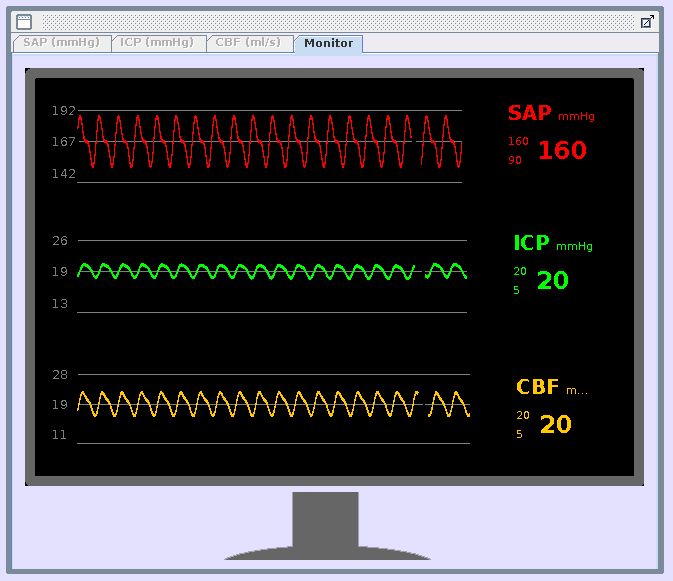
\includegraphics[width=\textwidth]{images/Q3C-Normal.png}
            \caption{Hemmorhage on normal brain}
    \end{minipage}
    \begin{minipage}{0.45\textwidth}
            \centering
            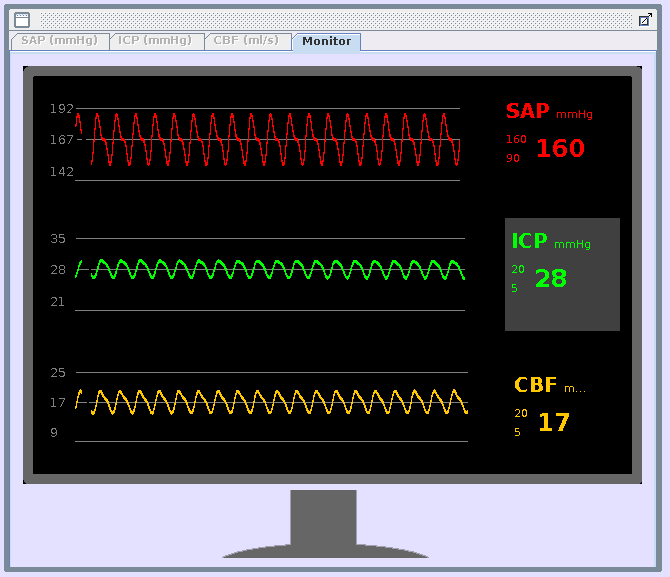
\includegraphics[width=\textwidth]{images/Q3C-TBI.png}
            \caption{10ml hemorrhage. Brain injury -- kRo: 3. kGaut: 0.5}
    \end{minipage}
\end{figure}

